\section{Auswertung}
\label{sec:Auswertung}
\subsection{Bestimmung der Winkelrichtgröße $D$ und des Trägheitsmoments
$I_\text{D}$ der Drillachse}
Zunächst werden die Konstanten der Apparatur, die Winkelrichtgröße $D$ und das
Eigenträgheitsmoment $I_\text{D}$ der Drillachse, bestimmt. Die Winkelrichtgröße
wird sowohl mit einer statischen Methode als auch mit einer dynamischen Methode
bestimmt, das Eigenträgheitsmoment nur mit der dynamischen Methode.

\subsubsection{statische Methode}
Mit einem Federkraftmesser wird die Rückstellkraft $F$ der Torsionsfeder bei festem
Abstand $r$ von der Drehachse in Abhängigkeit des Drehwinkels $\varphi$ gemessen.
Die Messwerte sowie die nach Gleichung (xx) berechnete Winkelrichtgröße $D$ sind
in Tabelle \ref{tab:statisch} zu aufgeführt.
\begin{table}[H]
  \centering
  \begin{tabular}{c c c c}
    \toprule
    \multicolumn{2}{c}{Drehwinkel $\varphi$} & $F$ in \si{\newton} & $D$ in \si{\newton\meter} \\
    in \si{\degree} & in \si{\radian} & & \\
    \midrule
    90  & 1.571 & 0.28 & 0.02653 \\
    100 & 1.745 & 0.30 & 0.02558 \\
    120 & 2.094 & 0.38 & 0.02700 \\
    150 & 2.618 & 0.49 & 0.02785 \\
    180 & 3.142 & 0.57 & 0.02700 \\
    200 & 3.491 & 0.61 & 0.02601 \\
    230 & 4.014 & 0.70 & 0.02595 \\
    270 & 4.712 & 0.80 & 0.02526 \\
    300 & 5.236 & 0.90 & 0.02558 \\
    330 & 5.760 & 1.00 & 0.02584 \\
    \bottomrule
  \end{tabular}
  \caption{Messwerte zur Berechnung der Winkelrichtgröße $D$ mit der statischen
  Methode.}
  \label{tab:statisch}
\end{table}
Für die Drehwinkel wird ein Ablesefehler von $\SI{5}{\degree} = \SI{0.087}{\radian}$
angenommen. Es wird der Mittelwert der Winkelrichtgröße nach Gleichung
\eqref{eqn:mittelwert} berechnet. Der Fehler ergibt sich mit Gaußscher
Fehlerfortpflanzung wie in Gleichung \eqref{eqn:fehlerfortpflanzung}. Damit ergibt
sich für die Winkelrichtgröße nach der statischen Methode
\begin{align*}
  D_\text{stat} = \SI{0.0263(3)}{\newton\meter}.
\end{align*}

\subsubsection{dynamische Methode}
Bei der dynamischen Methode wird die Schwingungsdauer $T$ für verschiedene Abstände
$a$ der Massen von der Drehachse gemessen. Die Messwerte sind in Tabelle
\ref{tab:dynamisch} dargestellt. Es wird $T^2$ gegen $a^2$ aufgetragen (siehe
Grafik \ref{fig:linreg_dynamisch}) und eine lineare Regression der Form
$y = b \cdot x + c$ mit Python durchgeführt.
\begin{figure}[H]
  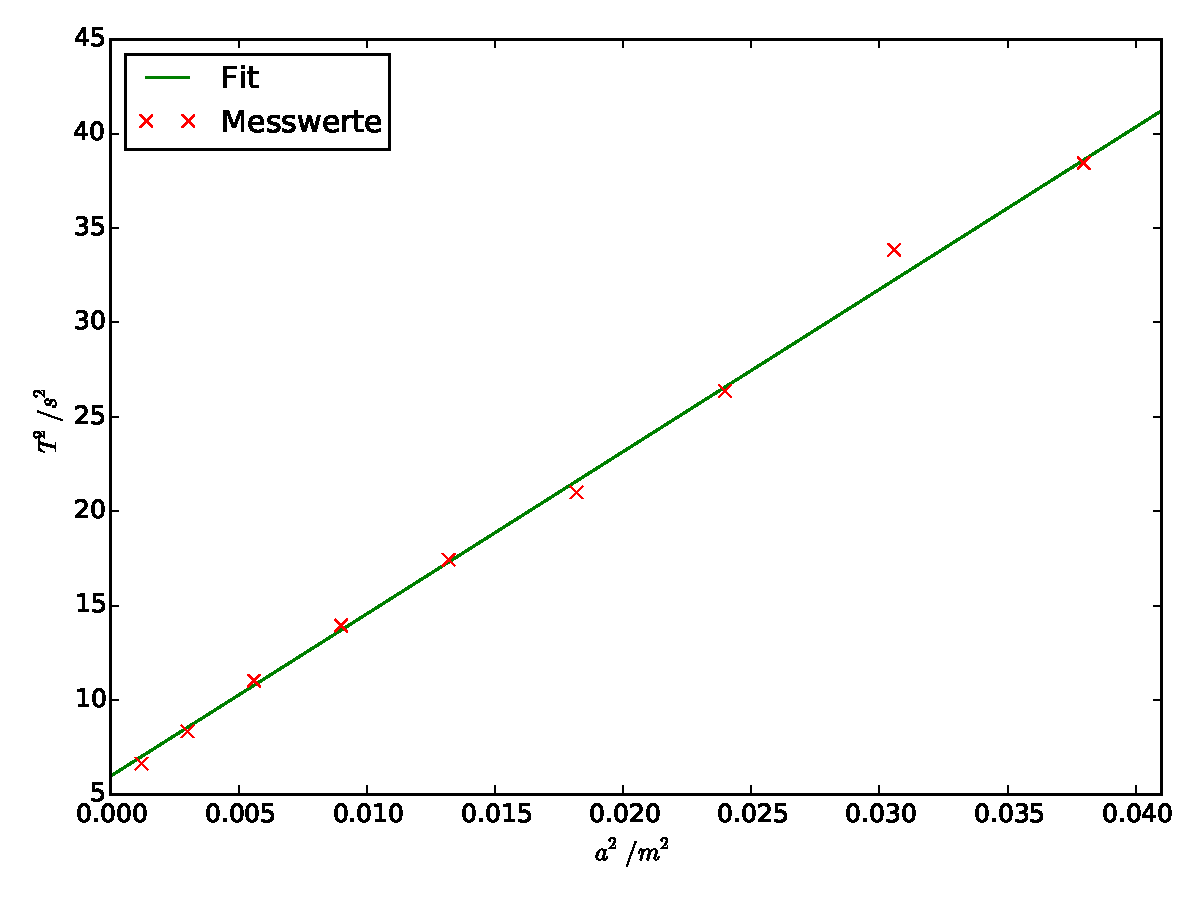
\includegraphics[width=0.8\textwidth]{dynamisch.pdf}
  \caption{Graph zur linearen Ausgleichsrechnung nach Gleichung
  \eqref{eqn:ausgleichsrechnung}.}
\end{figure}
Dies liefert mit den Messwerten aus Tabelle \ref{tab:messwerte_dynamisch} die
Parameter
\begin{align*}
  b &= \SI{860(15)}{\squared\second\per\squared\meter} \\
  c &= \SI{6.0(4)}{\squared\second}.
\end{align*}
\begin{table}
  \centering
  \begin{tabular}{c c c}
    \toprule
    Abstand $a$ in \si{\centi\meter} & \multicolumn{2}{c}{Schwingungsdauer T in \si{\second}} \\
     & 5 Perioden & 1 Periode \\
    \midrule
    3.485  & 12.87 & 2.574 \\
    5.485  & 14.44 & 2.888 \\
    7.485  & 16.60 & 3.320 \\
    9.485  & 18.67 & 3.734 \\
    11.485 & 20.87 & 4.174 \\
    13.485 & 22.91 & 4.582 \\
    15.485 & 25.67 & 5.134 \\
    17.485 & 29.09 & 5.818 \\
    19.485 & 31.00 & 6.200 \\
    21.485 & 33.53 & 6.706 \\
    \bottomrule
    \end{tabular}
  \caption{Messwerte der dynamischen Methode zur Berechnung von $D$ und
  $I_\text{D}$.}
  \label{tab:messwerte_dynamisch}
\end{table}

Die Gleichung (xx) lässt sich mit dem Gesamträgheitsmoment $I_\text{ges} =
I_\text{D} + I_\text{Z1} + I_\text{Z2}$ und den Trägheitsmomenten der Zylinder,
\begin{align*}
  I_\text{Z1} &= m_1 \left(\frac{R_1^2}{4}+\frac{h_1^2}{12}\right)+m_1 a^2 \text{ und }\\
  I_\text{Z1} &= m_2 \left(\frac{R_2^2}{4}+\frac{h_2^2}{12}\right)+m_2 a^2
\end{align*}
die um den Abstand $a$ von der Schwerpunktsachse verschoben sind, zu
\begin{align}
  T^2 &= 4 \pi^2 \frac{(m_1 + m_2)}{D} & a^2 &+ 4 \pi^2 \, \frac{m_1\left(
  \frac{R_1^2}{4} + \frac{h_1^2}{12}\right) + m_2 \left(\frac{R_2^2}{4}
  +\frac{h_2^2}{12}\right)+ I_\text{D}}{D}\\
  y &= b & x & + c
  \label{eqn:ausgleichsrechnung}
\end{align}
umformen.
Die Winkelrichtgröße wird dann mit der Gleichung
\begin{equation}
  D_\text{dyn} = 4 \pi^2 \frac{(m_1 + m_2)}{b}
  \label{eqn:D_dyn}
\end{equation}
berechnet und es ergibt sich mit Fehlerrechnung durch Python, der Steigung $b$
der linearen Regression und den Massen $m_1$ und $m_2$ aus der Tabelle
\ref{tab:gewichte}
\begin{align*}
  D_\text{dyn} = \SI{0.0205(4)}{\newton\meter}.
\end{align*}

\begin{table}
  \centering
  \begin{tabular}{c| c c}
    \toprule
        & Gewicht 1 (Zylinder) & Gewicht 2 (Zylinder)\\
    \midrule
    Masse $m$ in \si{\gram} & 223.43 & 222.50\\
    & & \\
    Durchmesser          & 3.45 & 3.46  \\
    in \si{\centi\meter} & 3.45 & 3.49  \\
                         & 3.44 & 3.48  \\
                         & 3.44 & 3.47  \\
                         & 3.45 & 3.475 \\
    & & \\
    Höhe                 & 2.97 & 2.975 \\
    in \si{\centi\meter} & 2.975 & 2.97 \\
                         & 2.97 & 2.975 \\
    \bottomrule
  \end{tabular}
  \caption{Abmessungen der zwei verwendeten Gewichte (beides Zylinder).}
  \label{tab:gewichte}
\end{table}

Das Eigenträgheitsmoment wird aus dem y-Achsenabschnitt der linearen
Ausgleichsrechnung \eqref{eqn:ausgleichsrechnung} mit der Gleichung
\begin{equation}
  I_\text{D} = m_1\left(\frac{R_1^2}{4} + \frac{h_1^2}{12}\right) + m_2 \left(
  \frac{R_2^2}{4}+\frac{h_2^2}{12}\right) - \frac{c}{b}\, (m_1 + m_2)
  \label{eqn:eigentraegheitsmoment}
\end{equation}
berechnet. Mit den Werten aus Tabelle \ref{tab:gewichte}, aus der sich insbesondere
die Radien
\begin{align*}
  R_1 &= \SI{0.01723(1)}{\meter} \text{ und }\\
  R_2 &= \SI{0.01737(3)}{\meter}
\end{align*}
und die Höhen der Zylinder
\begin{align*}
  h_1 &= \SI{0.02972(2)}{\meter} \text{ und } \\
  h_2 &= \SI{0.02973(2)}{\meter}
\end{align*}
ergeben, und den Parametern $b$ und $c$ der linearen Ausgleichsrechnung sowie
Fehlerfortpflanzung mit Python folgt für das Eigenträgheitsmoment
\begin{align*}
  I_\text{D} = \SI{-3.0(2)e-3}{\kilo\gram\squared\meter}.
\end{align*}
